%%%%%%%%%%%%%%%%%%%%%%%%%%%%%%%%%%%%%%%%%%%%%%%%%%%%%%%
%                File: OpEx_temp.tex                  %
%                  Date: Sept. 2, 2009                %
%                                                     %
%           LaTeX template file for use with          %
%           OSA's journal Optics Express              %
%                                                     %
%  send comments to Jennifer Mayfield, jmayfi@osa.org %
%                                                     %
% This file requires style file, opex3.sty, under     %
%              the LaTeX article class                %
%                                                     %
%   \documentclass[10pt,letterpaper]{article}         %
%   \usepackage{opex3}                                %
%                                                     %
% Note that our online submission system does not     %
% currently process PDFLaTeX; if PDFLaTeX must be     %
% used, pls. contact OpEx staff, and we will process  %
% manually                                            %
%                                                     %
%                                                     %
%       (c) 2009 Optical Society of America           %
%%%%%%%%%%%%%%%%%%%%%%%%%%%%%%%%%%%%%%%%%%%%%%%%%%%%%%%

%%%%%%%%%%%%%%%%%%%%%%% preamble %%%%%%%%%%%%%%%%%%%%%%%%%%%
\documentclass[10pt,letterpaper]{article}
\usepackage{opex3}
\graphicspath{{./Pictures/}}
\usepackage{caption}
\usepackage{subcaption}
\usepackage{amsmath} % Required for equation and aligned environments

 %\usepackage{ae} %%for Computer Modern fonts

%%%%%%%%%%%%%%%%%%%%%%% begin %%%%%%%%%%%%%%%%%%%%%%%%%%%%%%
\begin{document}

%%%%%%%%%%%%%%%%%% title page information %%%%%%%%%%%%%%%%%%
\title{Subpixel super resolution algorithm for \textit{PALM microscopy}}

\author{M. Gostiaux Gabriel}

\address{M. Gabriel Gostiaux, Master of Science student, Institute of Optics, \\ Palaiseau, 91 120, France}

\email{gabriel.gostiaux@institutoptique.fr} %% email address is required

\homepage{https://github.com/GabrielGst?tab=repositories} %% author's URL, if desired

%%%%%%%%%%%%%%%%%%% abstract and OCIS codes %%%%%%%%%%%%%%%%
%% [use \begin{abstract*}...\end{abstract*} if exempt from copyright]

\begin{abstract*}
In this study, we introduce a computationally efficient approach for generating super-resolution frames in Photoactivated Localization Microscopy (PALM) by accelerating the processing pipeline. The method is designed to optimize both the localization accuracy and processing speed, making it particularly suitable for medium-large datasets.

Our results demonstrate that this streamlined approach achieves robust performance in generating super-resolution PALM frames with significant reductions in processing time compared to the basic method, making it a good start for high-throughput super-resolution imaging applications.

\textbf{Keywords:} PALM Microscopy, sub-pixel superresolution, python. 

\end{abstract*}

\ocis{(000.0000) General.} % REPLACE WITH CORRECT OCIS CODES FOR YOUR ARTICLE

%%%%%%%%%%%%%%%%%%%%%%% References %%%%%%%%%%%%%%%%%%%%%%%%%
\begin{thebibliography}{99}

\bibitem{gallo99} K. Gallo and G. Assanto, ``All-optical diode based on second-harmonic generation in an asymmetric waveguide,'' \josab {\bf 16,} 267--269 (1999).

\end{thebibliography}

%%%%%%%%%%%%%%%%%%%%%%%%%%  body  %%%%%%%%%%%%%%%%%%%%%%%%%%
\section{Introduction}
PALM (Photoactivated Localization Microscopy) is a high-resolution imaging technique that surpasses the diffraction limit. It relies on the isolation of emitters selectively tagged with a fluorescent molecule, and the fitting of their Point Spread Function (PSF). The fluorescent molecules emit light when stimulated by a laser. This approach enables the precise localization of isolated emitters with an accuracy beyond the Rayleigh criterion, thus providing "super-resolution" down to around 10 nm. This technique, developed by Eric Betzig and his team in 2006, was awarded the Nobel Prize in Chemistry in 2014. It is of great importance due to its ability to enhance the resolution of existing images. Because this method is implemented with noisy frames, one should rely on estimation and detection theory to retrieve the precise coordinates of the emitters.

The workflow begins with a rigorous noise analysis of acquired frames, enabling the subsequent likelyhood computation steps to operate with enhanced precision. Our algorithm leverages a matched filter for likelihood calculation across frames, a critical step in improving computation time.

To accelerate the localization process, we identify initial guesses for molecule positions using a simple peak detection strategy via the numpy.max function. This initial estimation significantly reduces the computational complexity at the cost of sacrificing accuracy. For precise sub-pixel localization, we then employ the Maximum Likelihood Estimator (MLE) method, with optimization executed through the scipy.fmin function. This choice provides a computational efficiency and high-resolution localization, as it can then swiftly converges to optimal coordinates.

\section{Precision analysis}

For simplicity reasons and without any loss of generality, we consider the location from a 1D point of view. Let $x$ be the spatial coordinate, $\theta$ the position of an emitter. It is then assumed that the signal given by this single emitter on the image plan can be written as $s(x, \theta)=a r(x, \theta)+b$ where $r$ is a Gaussian function centered on $\theta$ so that

\begin{equation}
     r(x, \theta)=\frac{1}{\sqrt{2 \pi} \sigma_{r}} \exp \left[-\frac{(x-\theta)^{2}}{2 \sigma_{r}^{2}}\right]     
\end{equation}


where $\sigma_{r}$ is expressed as a function of the full width at half maximum (FWHM) $w$ of the signal on the sensor. In this labwork, $b$ is assumed to be an additive normal white noise of standard deviation $\sigma_{b}$.

P1 We define $r_{i}$ the integration of $r(x, \theta)$ over the pixel $i$ with $i \in[0, N-1]$


\begin{equation}
     r_{i}=\int_{i \Delta x}^{(i+1) \Delta x} r(x, \theta) \mathrm{d} x
\end{equation}


where $\Delta x$ is the discretization step. Give the expression of $r_{i}$ as a function of the parameters $\theta$ and $w$. We remind that


\begin{equation*}
\frac{2}{\sqrt{\pi}} \int_{0}^{z} e^{-u^{2}} \mathrm{~d} u=\operatorname{erf}(z)
\end{equation*}


Let's compute $r_i$ with a integration by substitution :


\begin{align}
     r_i & =\int_{i \Delta x}^{(i+1) \Delta x} \frac{1}{\sqrt{2 \pi} \sigma_r} \times \exp \left[-\left(\frac{x-\theta}{\sqrt{2} \sigma_r}\right)^2\right] d x \\
     & =\frac{1}{\sqrt{2 \pi} \sigma_r} \times \sqrt{2} \sigma_r \int_{u^{-}}^{u^{+}} e^{-u^2} d u \\
     & =\frac{1}{\sqrt{\pi}}\left[\int_0^{u^{+}} e^{-u^2} d u-\int_0^{u^{-}} e^{-u^2} d u\right]
\end{align}

\begin{align}
r_i= & \frac{1}{2}\left[\operatorname{erf}\left[\frac{(i+1) \Delta x-\theta}{\sqrt{2} \sigma_r}\right]-\operatorname{erf}\left[\frac{i \Delta x-\theta}{\sqrt{2} \sigma_r}\right]\right]
\end{align}


\begin{align}
P\left(s_{;}\right) &=\frac{1}{\sqrt{2 \pi} \sigma_b} \exp \left[-\frac{\left(s_i-a r_i\right)^2}{2 \sigma_b^2}\right] \\ 
l_\theta &=-N \times ln\left(\sqrt{2 \pi} \sigma_b\right) - \frac{1}{2 \sigma_b^2} \sum_{s_i  \in \Omega} \left(s_i-a r_i\right)^2 \\ 
\frac{\partial l_\theta}{\partial \theta} &=\frac{1}{\sigma_b^2} \sum_{s_i \in \Omega}\left(s_i-a r_i\right) \times a \times \frac{\partial r_i}{\partial \theta} 
\end{align}


\begin{equation}
     \frac{\partial r_i}{\partial \theta}=-\frac{1}{\sqrt{2 \pi} \sigma_r} \times\left[\exp -\left(\frac{(i+1) \Delta x-\theta}{\sqrt{2} \sigma_r}\right)^2-\exp -\left(\frac{i\Delta x-\theta}{\sqrt{2} \sigma_r}\right)^2\right]
\end{equation}

\begin{align}
\frac{\partial^2 l_\theta}{\partial^2 \theta} &=-\frac{1}{\sigma_b^2} \sum_{s_i \in \Omega}\left(-a\left(\frac{\partial c_i}{\partial \theta}\right)^2-\left(s_i-r_i\right) \frac{\partial^2 r_i}{\partial^2 \theta}\right) \\
\left\langle\frac{\partial^2 l_\theta}{\partial^2 \theta}\right\rangle &=-\frac{1}{\sigma_b^2} \sum_{s_i \in \Omega}\left(-a\left(\frac{\partial r_i}{\partial \theta}\right)^2-\left(\left\langle s_i\right\rangle-\alpha r_i\right) \frac{\partial^2 l_\theta}{\partial^2 \theta}\right) \\
\left\langle\frac{\partial^2 l_\theta}{\partial^2 \theta}\right\rangle &=\frac{a}{\sigma_b^2} \sum_{s_i \in \Omega}\left(\frac{\partial r_i}{\partial \theta}\right)^2
\end{align}



\begin{align}
& C R L B=-\frac{\sigma_b^2}{1} \times\left(\sum_{s_i \in \Omega} \left(\frac{\partial r_i}{\partial \theta}\right)^2\right)^{-1} \\
& C R L B=2\pi\sigma_b^2\sigma_r^2 \times\left(\sum_{s_i \in \Omega}\left(e^{-u_+^2}-e^{-u_{-}^2}\right)^2\right)^{-1}
\end{align}


\begin{figure}[h]
	\centering
	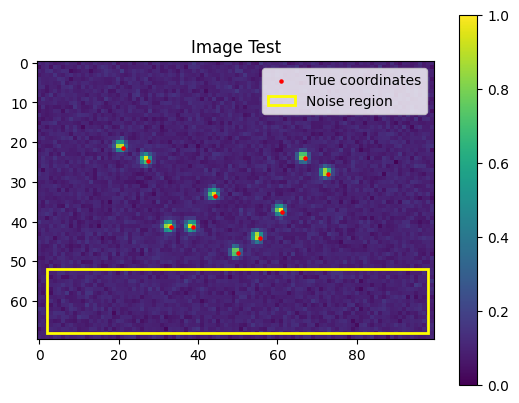
\includegraphics[scale=0.65]{image-test.png}
	\caption{Test Image}
	\label{fig:test}
\end{figure}

\begin{figure}[h]
     \centering
     \subfloat[Noise ]{
         \centering
         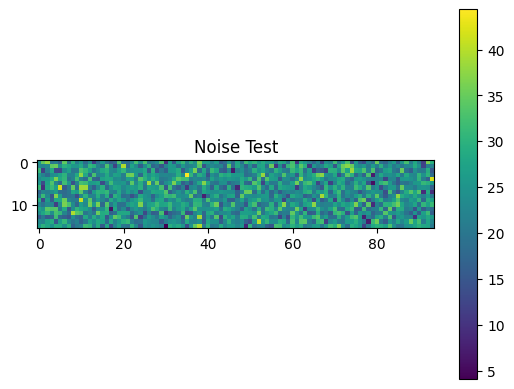
\includegraphics[width=0.45\textwidth]{noise.png}
         \label{fig:noise}
     }
      \subfloat[Noise 1D]{
          \centering
         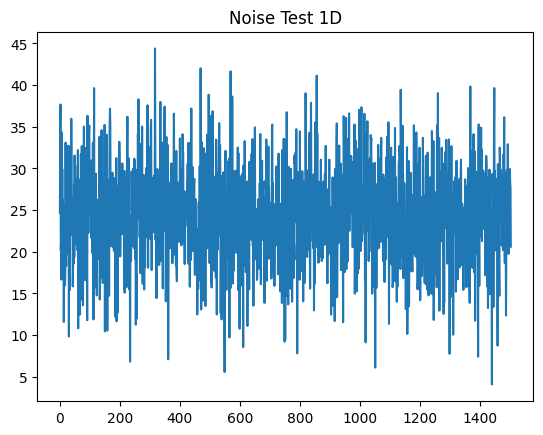
\includegraphics[width=0.45\textwidth]{noise-1D.png}
         \label{fig:noise-1D}
     }
     \caption{Noise}
\end{figure}

\begin{figure}[h]
     \centering
     \subfloat[Noise histogram]{
         \centering
         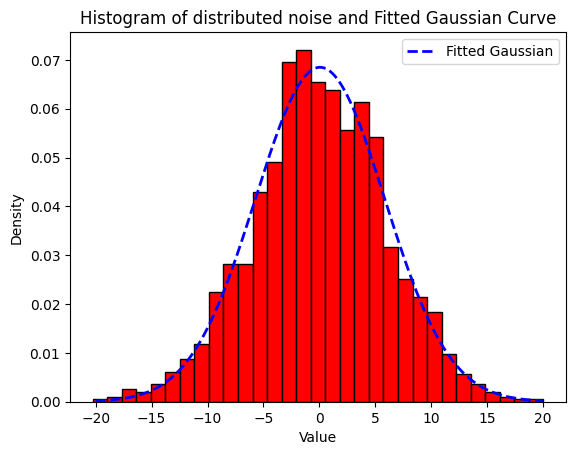
\includegraphics[width=0.45\textwidth]{fitted-gaussian-noise.png}
         \label{fig:fitted}
     }
      \subfloat[Noise correlation]{
          \centering
         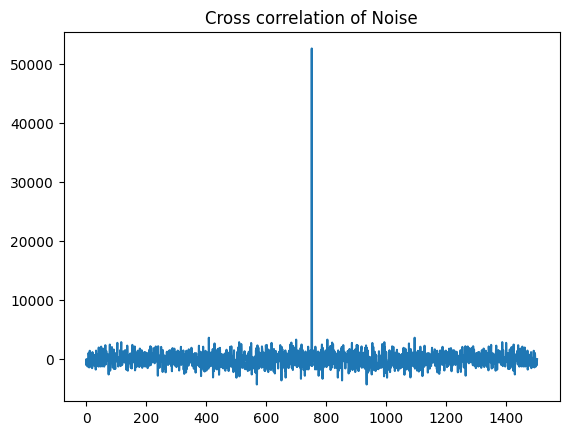
\includegraphics[width=0.45\textwidth]{correlation.png}
         \label{fig:correlation}
     }
     \caption{Noise properties}
\end{figure}

\section{Implementation of the algorithm}
\begin{figure}[h]
	\centering
	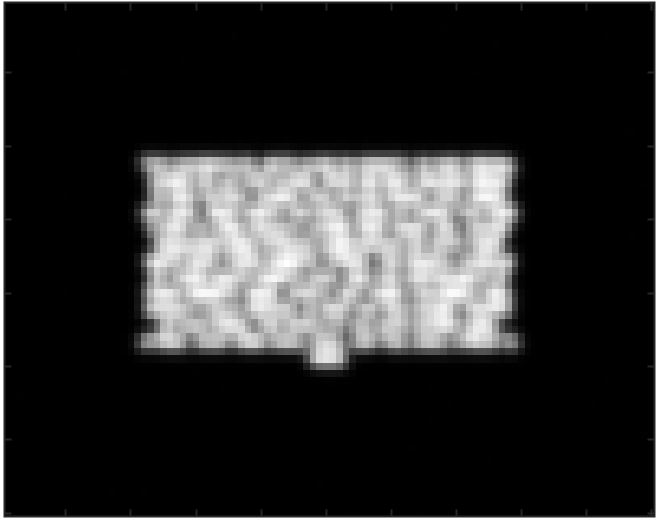
\includegraphics[scale=0.65]{ImageFloue.JPG}
	\caption{Image floue}
	\label{fig:floue}
\end{figure}


\begin{figure}[h]
	\centering
	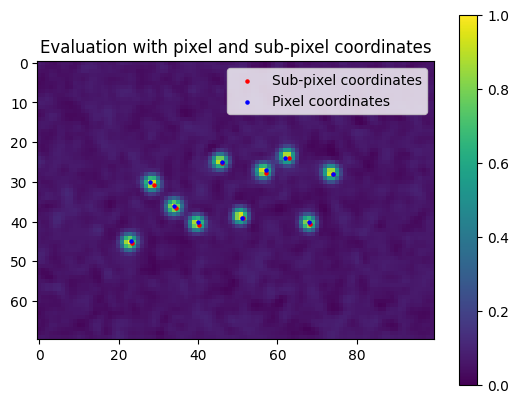
\includegraphics[scale=0.65]{evaluation of algo.png}
	\caption{Evaluation of algorithm acccuracy}
	\label{fig:eval}
\end{figure}


\begin{figure}[h]
     \centering
     \subfloat[Initial guesses]{
         \centering
         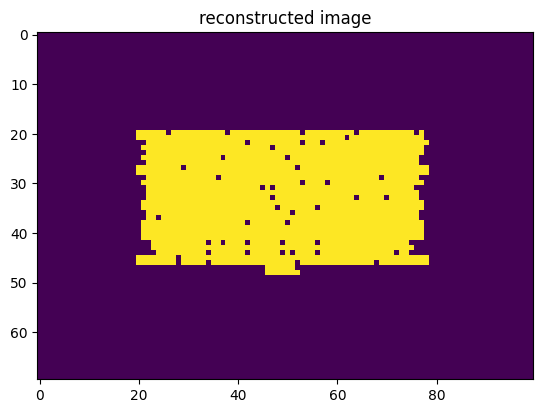
\includegraphics[width=0.45\textwidth]{pix-sum.png}
         \label{fig:pix}
     }
      \subfloat[Solving...]{
          \centering
         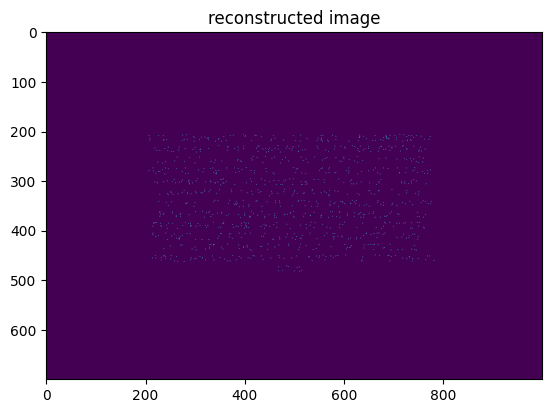
\includegraphics[width=0.45\textwidth]{solving-1.png}
         \label{fig:subpix}
     }
     \caption{Computing pix and subpix coordinates}
\end{figure}

\begin{figure}[h]
	\centering
	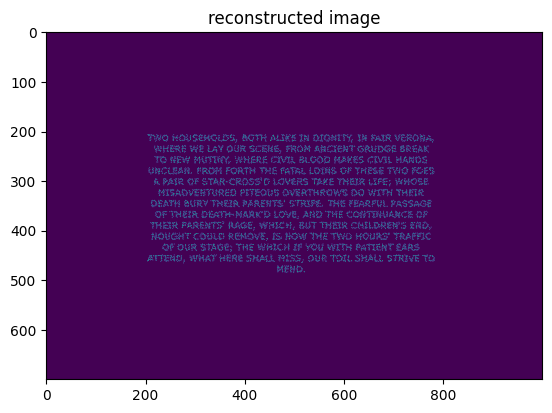
\includegraphics[scale=0.65]{solved text.png}
	\caption{Super resolution image}
	\label{fig:super}
\end{figure}

\section{Conclusion}
This study presented a specific workflow to optimize computation time for PALM microscopy. The proposed method consist in using a matched filter to compute and save the log-likelyhood arrays from the acquired frames, then use the numpy max function on those to find pixel-wide initial guesses for the scipy fmin optimization function. The time efficiency is then improved by a factor of 10, leading to compute the super-resoluted image presented at the end of section 2 in 10 minutes, while it was expected to be computed in 100 minutes with the basic fmin MLE optimization method.

The workflow produces a super-resoluted image on which one could read a passage of the famous "Romeo and Juliette" piece written by M. William Shakespeare, proving the accuracy of the method.

\end{document} 
